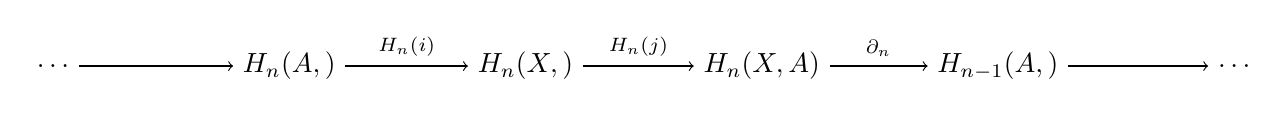
\begin{tikzpicture}

	\node (0) at (0,0) {$\ldots$};
	\node (1) at (3,0) {$H_n(A,\varnothing)$};
	\node (2) at (6,0) {$H_n(X,\varnothing)$};
	\node (3) at (9,0) {$H_n(X,A)$};
	\node (4) at (12,0) {$H_{n-1}(A,\varnothing)$};
	\node (5) at (15,0) {$\ldots$};
	
	\path[->, font=\scriptsize]
		(0) edge (1)
		(1) edge node[above]{$H_n(i)$} (2)
		(2) edge node[above]{$H_n(j)$} (3)
		(3) edge node[above]{$\partial_n$} (4)
		(4) edge (5);

\end{tikzpicture}